% Appendices, shared by main.tex and imc.tex. IMC requires the Ethics, Open
% Science and Generative AI sections.
\section{Ethics}
\label{sec:ethics}

This work involves no human subjects. 
The RQ2 probes are the unauthenticated handshakes a browser starts. Each
endpoint received the probe's ClientHello and one standard handshake, each
retried a bounded number of times on failure, and no application data. The global rate was
\data{rqtwo-rate} connections per second and at most one connection per host
was open at a time, both enforced in code. Nothing was exploited and no
credentials were tried. The project's documentation describes exactly what a
probe sends and how to opt out; the opt-out list is honoured by every run and
held \data{rqtwo-exclude} entries at the time of the scan. We report results
in aggregate and will report notable findings about federal systems through
CISA. The scanning source address has no reverse DNS record pointing to the
project, which we note as a shortcoming of this run. RQ3 clones public
repositories and runs none of their code. These practices follow the
recommendations of the ZMap authors~\cite{zmap} and the Menlo
Report~\cite{menlo}.


\section{Open Science}

Every artifact behind this paper is public: \tool{}'s source under the
Apache~2.0 license, the labeled corpus and the evaluation harness with every
competitor pinned by image digest, the measurement and benchmark scripts, the
raw measurement data (every probe record of RQ2 and every finding of RQ3),
and this paper's generator, at \artifactlink. Every number, table and figure is generated from the files in
\texttt{paper/data} by \texttt{paper/gen.py}, and a check fails the build if
any digit is typed into the paper's sources. The data come from these runs:
\begin{itemize}
\item RQ1: \texttt{make eval}, with competitors pinned by image digest.
\item RQ2: \texttt{measure/rq2.sh}, at \tool{} revision
  \rev{\data{rqtwo-revision}}, CISA list commit
  \texttt{\data{rqtwo-dotgov-commit}}, on \data{rqtwo-date}.
\item RQ3: \texttt{measure/rq3.sh}, at revision
  \rev{\data{rqthree-revision}}, Criticality Score snapshot
  \data{rqthree-snapshot} from commit
  \texttt{\data{rqthree-criticality-commit}}.
\item RQ4: \texttt{make bench}, at revision \rev{\data{rqfour-revision}},
  on \data{rqfour-date}.
\item RQ5: \texttt{measure/\allowbreak fed\_link.py} and
  \texttt{measure/\allowbreak fed\_scan.py},
  on \data{fed-date}, with GitHub's government registry at commit
  \texttt{\data{fed-registry-commit}} and the RQ2 records as the deployed side.
\item Risk-score ablation: \texttt{make risk-ablation}, at revision
  \rev{\data{riskabl-revision}}, from the RQ3 findings.
\end{itemize}

\section{Generative AI}

\textbf{[To be completed by the author before submission: state which
generative AI tools were used in this work, for what (for example writing
code, analysis scripts, or drafting and editing text), and how their output
was checked.]}

\section{Emulated-Link Handshakes}
\label{app:netem}

Table~\ref{tab:rq4-tls} and Figure~\ref{fig:rq4-extra} give the handshake
timings under emulated delay and loss that \S\ref{sec:rq4} sets aside. The
links were emulated with \texttt{netem} on the loopback interface of a Linux
container running in a virtual machine on the host of
Table~\ref{tab:rq4-primitives}. The hybrid's extra median time does not scale
with the added round-trip time, and we have not found the cause, so these
numbers should not be read as wide-area costs.

\begin{table*}[t]
\centering\small
% Generated by paper/gen.py from paper/data. Do not edit.
\begin{tabular}{lrrrrrrrr}
\toprule
Profile & $n$ & \multicolumn{3}{c}{p50 handshake} & \multicolumn{2}{c}{Hybrid extra} & \multicolumn{2}{c}{p99} \\
\cmidrule(lr){3-5}\cmidrule(lr){6-7}\cmidrule(lr){8-9}
 &  & X25519 & Hybrid & Go def. & abs. & rel. & X25519 & Hybrid \\
\midrule
loopback & 200 & 0.31\,ms & 0.46\,ms & 0.45\,ms & 0.15\,ms & 48\% & 0.98\,ms & 1.48\,ms \\
loopback, MTU 1500 & 200 & 0.31\,ms & 0.46\,ms & 0.46\,ms & 0.15\,ms & 50\% & 0.60\,ms & 0.97\,ms \\
+2\,ms RTT & 200 & 4.74\,ms & 6.04\,ms & 5.92\,ms & 1.30\,ms & 28\% & 7.08\,ms & 7.86\,ms \\
+40\,ms RTT & 200 & 50.42\,ms & 51.77\,ms & 51.87\,ms & 1.35\,ms & 3\% & 61.15\,ms & 62.31\,ms \\
+40\,ms RTT, 1\% loss & 500 & 50.99\,ms & 51.17\,ms & 52.03\,ms & 0.18\,ms & 0\% & 320.28\,ms & 312.32\,ms \\
+150\,ms RTT & 200 & 163.44\,ms & 164.64\,ms & 164.61\,ms & 1.20\,ms & 1\% & 173.02\,ms & 173.51\,ms \\
\bottomrule
\end{tabular}

\caption{Full TLS~1.3 handshake time in the Linux container under each
\texttt{netem} profile, from established TCP connection to usable TLS
connection: medians for the X25519-only, hybrid-only and Go default
clients, the hybrid's extra median time over X25519, and p99.}
\label{tab:rq4-tls}
\end{table*}

\begin{figure}[t]
\centering
% Generated by paper/gen.py from paper/data. Do not edit.
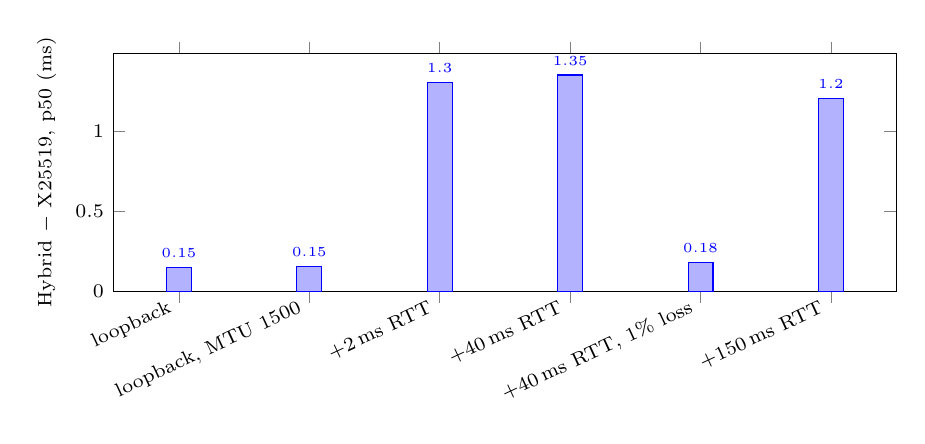
\begin{tikzpicture}
\begin{axis}[
  ybar, ymin=0, width=0.95\linewidth, height=4.6cm, bar width=9pt,
  symbolic x coords={{loopback},{loopback, MTU 1500},{+2\,ms RTT},{+40\,ms RTT},{+40\,ms RTT, 1\% loss},{+150\,ms RTT}}, xtick=data,
  x tick label style={font=\scriptsize, rotate=25, anchor=east},
  y tick label style={font=\scriptsize}, label style={font=\scriptsize},
  ylabel={Hybrid $-$ X25519, p50 (ms)},
  nodes near coords, every node near coord/.append style={font=\tiny, /pgf/number format/.cd, fixed, precision=2},
]
\addplot coordinates {({loopback},0.148) ({loopback, MTU 1500},0.154) ({+2\,ms RTT},1.303) ({+40\,ms RTT},1.349) ({+40\,ms RTT, 1\% loss},0.180) ({+150\,ms RTT},1.204)};
\end{axis}
\end{tikzpicture}

\caption{Extra median handshake time of X25519MLKEM768 over X25519, per
\texttt{netem} profile.}
\label{fig:rq4-extra}
\end{figure}

\clearpage
\section{Additional Tables}

\begin{table}[!htbp]
\centering\footnotesize\setlength{\tabcolsep}{4pt}
% Generated by paper/gen.py from paper/data. Do not edit.
\begin{tabular}{p{0.46\linewidth}rrrr}
\toprule
Agency & TLS & Hyb. & Share & 95\% CI \\
\midrule
Consumer Product Safety Commission & 20 & 20 & 100.0\% & 84--100 \\
Federal Trade Commission & 28 & 28 & 100.0\% & 88--100 \\
Library of Congress & 58 & 58 & 100.0\% & 94--100 \\
Department of Homeland Security & 74 & 70 & 94.6\% & 87--98 \\
Office of the Director of National Intelligence & 20 & 18 & 90.0\% & 70--97 \\
Department of Labor & 49 & 43 & 87.8\% & 76--94 \\
National Archives and Records Administration & 62 & 51 & 82.3\% & 71--90 \\
Department of Justice & 101 & 83 & 82.2\% & 74--88 \\
Department of Transportation & 26 & 21 & 80.8\% & 62--91 \\
Department of Commerce & 109 & 81 & 74.3\% & 65--82 \\
Government Publishing Office & 28 & 19 & 67.9\% & 49--82 \\
Department of the Interior & 97 & 65 & 67.0\% & 57--76 \\
Department of State & 28 & 18 & 64.3\% & 46--79 \\
Department of Defense & 45 & 23 & 51.1\% & 37--65 \\
United States House of Representatives & 38 & 19 & 50.0\% & 35--65 \\
Department of Health and Human Services & 196 & 97 & 49.5\% & 43--56 \\
Department of Education & 20 & 9 & 45.0\% & 26--66 \\
General Services Administration & 131 & 51 & 38.9\% & 31--47 \\
Executive Office of the President & 103 & 37 & 35.9\% & 27--46 \\
Department of the Treasury & 121 & 43 & 35.5\% & 28--44 \\
Department of Energy & 81 & 23 & 28.4\% & 20--39 \\
Office of Personnel Management & 29 & 6 & 20.7\% & 10--38 \\
Department of Agriculture & 51 & 10 & 19.6\% & 11--32 \\
\bottomrule
\end{tabular}

\caption{Hybrid adoption for agencies with at least \data{rqtwo-agency-min}
TLS endpoints, with Wilson 95\% intervals.}
\label{tab:rq2-agencies}
\end{table}

\begin{table}[!htbp]
\centering\small
% Generated by paper/gen.py from paper/data. Do not edit.
\begin{tabular}{lrrr}
\toprule
Algorithm & Projects & Share & Findings \\
\midrule
RSA & 49 & 51\% & 4,611 \\
ECDSA & 34 & 35\% & 1,878 \\
EdDSA & 29 & 30\% & 334 \\
X25519 & 25 & 26\% & 286 \\
ECDH & 24 & 25\% & 261 \\
DSA & 23 & 24\% & 151 \\
DH & 14 & 14\% & 33 \\
X448 & 14 & 14\% & 42 \\
\bottomrule
\end{tabular}

\caption{Quantum-vulnerable algorithms in the \data{rqthree-scanned} scanned
projects: projects with at least one finding, and findings.}
\label{tab:rq3-algorithms}
\end{table}
